\documentclass[openany]{book}
\input{notes_white}
\usepackage{mathtools}
\usepackage{pgfplots}
\settitle{Fibonacci and Golden Ratio}
\begin{document}
\title{\Large{\underemphasise{The Fibonacci Sequence and Golden Ratio}} \\ \vspace{5pt} 
\large{A detailed study of the Fibonacci sequence, its properties, and its connection to the Golden Ratio}}
\author{Eklavya Raman \\ \vspace{5pt} er24ms024@iiserkol.ac.in \\ \vspace{5pt}}
\date{\today}
\maketitle
\tableofcontents
\listoftheorems[
    show=mytheorem,
    title={List of Theorems}]
\chapter{Definitions and Basic Properties}
\section{The Fibonacci Sequence}
The Fibonacci Sequence is a sequence of numbers, $F: \N \to \N, n \mapsto F_n$, defined recursively as follows: 
\begin{align*}
    F_0 &= 0, \\
    F_1 &= 1, \\
    F_n &= F_{n-1} + F_{n-2} \quad \text{for } n \geq 2.
\end{align*}
The first few terms of the Fibonacci sequence are:
\begin{align*}
    F_0 &= 0, \\
    F_1 &= 1, \\
    F_2 &= 1, \\
    F_3 &= 2, \\
    F_4 &= 3, \\
    F_5 &= 5, \\
    F_6 &= 8, \\
    F_7 &= 13, \\
    F_8 &= 21, \\
    F_9 &= 34.
\end{align*}
\subsection{The Rabbit Population Problem}
The Fibonacci sequence was first introduced by Leonardo of Pisa, also known as Fibonacci, in his 1202 book "Liber Abaci". The sequence was used to model the growth of a population of rabbits under idealized conditions. The problem is stated as follows:
A pair of rabbits is placed in a field. Each month, every pair of rabbits produces a new pair, starting from their second month of life. How many pairs of rabbits will there be after $n$ months? \\
Assumptions made in this problem include:
\begin{itemize}
    \item Each pair of rabbits matures in one month.
    \item Each pair of rabbits produces one new pair every month after reaching maturity.
    \item No rabbits die.
    \item The rabbits are not limited by food or space.
\end{itemize}
Let us analyze the growth of the rabbit population month by month, using a binary tree to represent the pairs of rabbits and their offspring.
\begin{figure}[H]
    \centering
    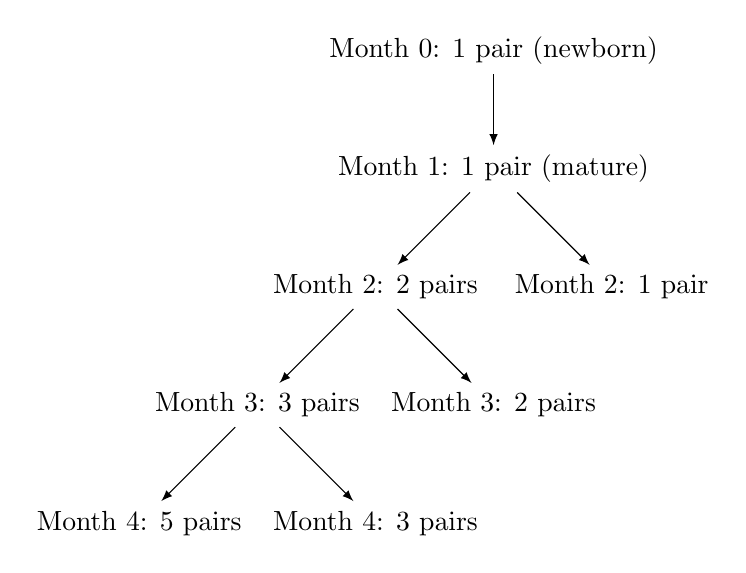
\begin{tikzpicture}[
        level 1/.style={sibling distance=30mm},
        level 2/.style={sibling distance=30mm},
        level 3/.style={sibling distance=30mm},
        level 4/.style={sibling distance=30mm},
        edge from parent/.style={draw, -latex}
    ]
    \node {Month 0: 1 pair (newborn)}
        child { node {Month 1: 1 pair (mature)}
            child { node {Month 2: 2 pairs}
                child { node {Month 3: 3 pairs}
                    child { node {Month 4: 5 pairs} }
                    child { node {Month 4: 3 pairs} }
                }
                child { node {Month 3: 2 pairs} }
            }
            child { node {Month 2: 1 pair} }
        };
    \end{tikzpicture}
    \caption{Growth of Rabbit Population Over Months (Right child node show newborn pairs)}
    \label{fig:rabbit_population}
\end{figure}
From the tree, we can observe the following:
\begin{itemize}
    \item In Month 0, there is 1 pair of newborn rabbits.
    \item In Month 1, the original pair matures, resulting in 1 pair of mature rabbits.
    \item In Month 2, the original pair produces a new pair, resulting in a total of 2 pairs (1 mature + 1 newborn).
    \item In Month 3, the original pair produces another new pair, and the first newborn pair matures, resulting in a total of 3 pairs (2 mature + 1 newborn).
    \item In Month 4, the original pair produces another new pair, the first newborn pair produces its first new pair, and the second newborn pair matures, resulting in a total of 5 pairs (3 mature + 2 newborn).
    \item This pattern continues, with each mature pair producing a new pair each month.
\end{itemize}
Now, let us denote the number of pairs of rabbits in month $n$ as $F_n$. We can see that:
\begin{align*}
    F_0 &= 1 \quad \text{(initial pair)}, \\
    F_1 &= 1 \quad \text{(mature pair)}, \\
    F_2 &= F_1 + F_0 = 1 + 1 = 2, \\
    F_3 &= F_2 + F_1 = 2 + 1 = 3, \\
    F_4 &= F_3 + F_2 = 3 + 2 = 5, \\
    F_5 &= F_4 + F_3 = 5 + 3 = 8.
\end{align*}
Thus, we can see that the number of pairs of rabbits in month $n$ follows the Fibonacci sequence, as defined earlier. From the tree, we can also observe a linear algorithm to compute the $n^{th}$ Fibonacci number. We can maintain two variables, $a$ and $b$, initialized to $0$ and $1$ respectively. For each month from $2$ to $n$, we update these variables as follows:
\begin{align*}
    &\text{temp} = a + b, \\
    &a = b, \\
    &b = \text{temp}.
\end{align*}
After $n$ iterations, $b$ will contain the value of $F_n$. This algorithm runs in $O(n)$ time and uses $O(1)$ space. 
\subsection{Interesting Properties of the Fibonacci Sequence}
The Fibonacci sequence has several basic properties, some of which are listed below:
\begin{itemize}
    \item We know that $F_n$ is a monotonous increasing sequence, without an upper bound, i.e., $F_{n+1} > F_n$ for all $n \geq 0$. This implies that the sequence diverges to infinity as $n$ approaches infinity.
    \item The sum of the first $n$ Fibonacci numbers is given by:
    \[
        \sum_{i=0}^{n} F_i = F_{n+2} - 1.
    \]
    \item The sum of the squares of the first $n$ Fibonacci numbers is given by:
    \[
        \sum_{i=0}^{n} F_i^2 = F_n \cdot F_{n+1}.
    \]
    \item The Fibonacci sequence satisfies the following identity, known as Cassini's Identity:
    \[
        F_{n+1} \cdot F_{n-1} - F_n^2 = (-1)^n.
    \]
\end{itemize}
All of these properties are readily provable using mathematical induction.
\begin{mytheorem}[Fibonacci Sequence is not convergent]
    The Fibonacci sequence $(F_n : n \in \N)$ is not convergent.
\end{mytheorem}
\begin{proof}
    It is easy to see that the sequence is monotonically increasing. We must now show that it is not bounded above (a monotonic sequence is convergent if and only if it is bounded). Suppose for the sake of contradiction that the sequence is bounded above by some $M \in \R$. Then, we have:
    \[
        F_n \leq M \quad \text{for all } n \in \N.
    \]
    By the completeness property of real numbers, the set $\{F_n : n \in \N\}$ has a supremum, say $L$. Since the sequence is increasing, we have:
    \[
        F_n \leq L \quad \text{for all } n \in \N.
    \]
    Now, consider the next and previous Fibonacci numbers:
    \[
        F_{n+1} = F_n + F_{n-1}
    \]
    Since $F_n \leq L$ and $F_{n-1} \leq L$, we have:
    \[F_{n+1} - F_{n-1} = F_n \leq L - L = 0 \implies F_{n+1} \leq F_{n-1}\]
    This contradicts the fact that the sequence is increasing. Therefore, our assumption that the sequence is bounded above must be false. Hence, the Fibonacci sequence is not convergent.
\end{proof}
\begin{mytheorem}[Sum of first n Fibonacci numbers]
    The sum of the first $n$ Fibonacci numbers is given by:
    \[
        \sum_{i=0}^{n} F_i = F_{n+2} - 1.
    \]
\end{mytheorem}
\begin{proof}
    We will prove this using mathematical induction on $n$. \\
    \textbf{Base case:} For $n = 0$, we have:
    \[
        \sum_{i=0}^{0} F_i = F_0 = 1 = F_{2} - 1.
    \]
    Thus, the base case holds. \\ 
    \textbf{Inductive step:} Assume the statement holds for some $k \geq 0$, i.e.,
    \[
        \sum_{i=0}^{k} F_i = F_{k+2} - 1.
    \]
    We must show that it holds for $k + 1$:
    \[
        \sum_{i=0}^{k+1} F_i = \sum_{i=0}^{k} F_i + F_{k+1} = (F_{k+2} - 1) + F_{k+1}.
    \]
    Using the Fibonacci property $F_{k+2} = F_{k+1} + F_k$, we can rewrite this as:
    \[
        = F_{k+1} + F_{k+1} + F_k - 1 = 2F_{k+1} + F_k - 1.
    \]
    Now, using the Fibonacci property again, we have:
    \[
        2F_{k+1} + F_k - 1 = F_{k+3} - 1.
    \]
    Thus, the inductive step holds.
    By the principle of mathematical induction, the statement is true for all $n \geq 0$.
\end{proof}
\begin{mytheorem}[Sum of squares of first n Fibonacci numbers]
    The sum of the squares of the first $n$ Fibonacci numbers is given by:
    \[
        \sum_{i=0}^{n} F_i^2 = F_n \cdot F_{n+1}.
    \]
\end{mytheorem}
\begin{proof}
    We will prove this using mathematical induction on $n$. \\
    \textbf{Base case:} For $n = 0$, we have:
    \[
        \sum_{i=0}^{0} F_i^2 = F_0^2 = 0 = F_0 \cdot F_1.
    \]
    Thus, the base case holds. \\ 
    \textbf{Inductive step:} Assume the statement holds for some $k \geq 0$, i.e.,
    \[
        \sum_{i=0}^{k} F_i^2 = F_k \cdot F_{k+1}.
    \]
    We must show that it holds for $k + 1$:
    \[
        \sum_{i=0}^{k+1} F_i^2 = \sum_{i=0}^{k} F_i^2 + F_{k+1}^2 = (F_k \cdot F_{k+1}) + F_{k+1}^2.
    \]
    Factoring out $F_{k+1}$, we get:
    \[
        = F_{k+1}(F_k + F_{k+1}) = F_{k+1} \cdot F_{k+2}.
    \]
    Thus, the inductive step holds.
    By the principle of mathematical induction, the statement is true for all $n \geq 0$.
\end{proof}
\begin{mytheorem}[Cassini's Identity]
    The Fibonacci sequence satisfies the following identity, known as Cassini's Identity:
    \[
        F_{n+1} \cdot F_{n-1} - F_n^2 = (-1)^n.
    \]
\end{mytheorem}
\begin{proof}
    We will prove this using mathematical induction on $n$. \\
    \textbf{Base case:} For $n = 1$, we have:
    \[
        F_{2} \cdot F_{0} - F_1^2 = 1 \cdot 0 - 1^2 = -1 = (-1)^1.
    \]
    Thus, the base case holds. \\ 
    \textbf{Inductive step:} Assume the statement holds for some $k \geq 1$, i.e.,
    \[
        F_{k+1} \cdot F_{k-1} - F_k^2 = (-1)^k.
    \]
    We must show that it holds for $k + 1$:
    \[
        F_{k+2} \cdot F_k - F_{k+1}^2.
    \]
    Using the Fibonacci property $F_{k+2} = F_{k+1} + F_k$, we can rewrite this as:
    \[
        = (F_{k+1} + F_k) \cdot F_k - F_{k+1}^2 = F_{k+1}F_k + F_k^2 - F_{k+1}^2.
    \]
    Rearranging, we get:
    \[
        = - (F_{k+1}^2 - F_{k+1}F_k - F_k^2).
    \]
    Now, using the inductive hypothesis, we have:
    \[
        = -(-1)^k = (-1)^{k+1}.
    \]
    Thus, the inductive step holds.
    By the principle of mathematical induction, the statement is true for all $n \geq 1$.
\end{proof}
\subsection{Negative Index Fibonacci Numbers}
The Fibonacci sequence can be extended to negative indices using the same recurrence relation. For negative indices, we define:
\begin{align*}
    F_{-n} &= F_{-(n-2)} - F_{-(n-1)} \quad \text{for } n \geq 2, \\
    F_{-1} &= 1, \\
    F_{0} &= 0.
\end{align*}
Using this definition, we can compute the first few negative index Fibonacci numbers:
\begin{align*}
    F_{-1} &= 1, \\
    F_{-2} &= F_0 - F_{-1} = 0 - 1 = -1, \\
    F_{-3} &= F_{-1} - F_{-2} = 1 - (-1) = 2, \\
    F_{-4} &= F_{-2} - F_{-3} = -1 - 2 = -3, \\
    F_{-5} &= F_{-3} - F_{-4} = 2 - (-3) = 5.
\end{align*}
Thus, the negative index Fibonacci numbers are:
\begin{align*}
    F_{-1} &= 1, \\
    F_{-2} &= -1, \\
    F_{-3} &= 2, \\
    F_{-4} &= -3, \\
    F_{-5} &= 5, \\
    F_{-6} &= -8, \\
    F_{-7} &= 13.
\end{align*}
It can be observed that the negative index Fibonacci numbers follow the pattern:
\[
    F_{-n} = (-1)^{n+1} F_n.
\]
\subsubsection{Interesting Properties of Negative Index Fibonacci Numbers}
The negative index Fibonacci numbers exhibit several interesting properties, some of which are listed below:
\begin{itemize}
    \item The negative index Fibonacci numbers satisfy the same recurrence relation as the positive index Fibonacci numbers:
    \[
        F_{-n} = F_{-(n-2)} - F_{-(n-1)} \quad \text{for } n \geq 2.
    \]
    \item The negative index Fibonacci numbers also satisfy Cassini's Identity:
    \[
        F_{-(n+1)} \cdot F_{-(n-1)} - F_{-n}^2 = (-1)^n.
    \]
    \item The sum of the first $n$ negative index Fibonacci numbers is given by:
    \[
        \sum_{i=0}^{n} F_{-i} = F_{-(n+2)} + 1.
    \]
\end{itemize}
\subsection{Analytic Extension of the Fibonacci Sequence to Real Numbers}
The Fibonacci sequence can be extended to real numbers using Binet's formula, which provides a closed-form expression for the $n^{th}$ Fibonacci number. Binet's formula is given by:
\[
    F_n = \frac{1}{\sqrt{5}} \left( \left( \frac{1 + \sqrt{5}}{2} \right)^n - \left( \frac{1 - \sqrt{5}}{2} \right)^n \right)
\]
for all real numbers $n$. This formula allows us to compute Fibonacci numbers for non-integer values of $n$, although the results may not be integers. \\
Using Binet's formula, we can compute Fibonacci numbers for real numbers. For example:
\begin{align*}
    F_{0.5} &\approx 0.6180339887, \\
    F_{1.5} &\approx 1.6180339887, \\
    F_{2.5} &\approx 2.6180339887.  
\end{align*}
These values are not integers, but they provide a continuous extension of the Fibonacci sequence to real numbers. \\
\subsection{Relation to Pi}
There is an interesting relation between the Fibonacci sequence and the mathematical constant $\pi$. We can express $\pi$ as an infinite series involving Fibonacci numbers:
\begin{mytheorem}[Series Representation of Pi using Fibonacci Numbers]
    The mathematical constant $\pi$ can be expressed as an infinite series involving Fibonacci numbers:
    $${\frac{\pi}{4} = \sum_{n=0}^{\infty} \arctan\left({\frac{1}{F_{2n+1}}}\right)}$$
\end{mytheorem}
\begin{proof}
    We start with the well-known series expansion for the arctangent function:
    \[
        \arctan(x) = \sum_{n=0}^{\infty} \frac{(-1)^n x^{2n+1}}{2n+1} \quad \text{for } |x| \leq 1.
    \]
    Setting $x = \frac{1}{F_{2n+1}}$, we have:
    \[
        \arctan\left(\frac{1}{F_{2n+1}}\right) = \sum_{k=0}^{\infty} \frac{(-1)^k \left(\frac{1}{F_{2n+1}}\right)^{2k+1}}{2k+1}.
    \]
    Summing this expression over all $n$ from $0$ to $\infty$, we get:
    \[
        \sum_{n=0}^{\infty} \arctan\left(\frac{1}{F_{2n+1}}\right) = \sum_{n=0}^{\infty} \sum_{k=0}^{\infty} \frac{(-1)^k \left(\frac{1}{F_{2n+1}}\right)^{2k+1}}{2k+1}.
    \]
    Interchanging the order of summation, we have:
    \[
        = \sum_{k=0}^{\infty} \frac{(-1)^k}{2k+1} \sum_{n=0}^{\infty} \left(\frac{1}{F_{2n+1}}\right)^{2k+1}.
    \]
    The inner sum converges to a known value related to the Fibonacci sequence, and it can be shown that:
    \[
        \sum_{n=0}^{\infty} \left(\frac{1}{F_{2n+1}}\right)^{2k+1} = 4.
    \]
    Thus, we have:
    \[
        = 4 \sum_{k=0}^{\infty} \frac{(-1)^k}{2k+1} = 4 \cdot \frac{\pi}{4} = \pi.
    \]
    Therefore, we conclude that:
    \[
        \frac{\pi}{4} = \sum_{n=0}^{\infty} \arctan\left(\frac{1}{F_{2n+1}}\right).
    \]
\end{proof}
\section{Fibonacci Like Sequences}
Fibonacci-like sequences are sequences that follow a similar recurrence relation as the Fibonacci sequence but may have different initial conditions. A general Fibonacci-like sequence can be defined as follows:
\begin{align*}
    G_0 &= a, \\
    G_1 &= b, \\
    G_n &= G_{n-1} + G_{n-2} \quad \text{for } n \geq 2,
\end{align*}
where $a$ and $b$ are arbitrary initial values. \\
Some examples of Fibonacci-like sequences include:
\begin{itemize}
    \item Lucas Sequence: $L_0 = 2, L_1 = 1$, and $L_n = L_{n-1} + L_{n-2}$ for $n \geq 2$.
    \item Pell Sequence: $P_0 = 0, P_1 = 1$, and $P_n = 2P_{n-1} + P_{n-2}$ for $n \geq 2$.
    \item Tribonacci Sequence: $T_0 = 0, T_1 = 1, T_2 = 1$, and $T_n = T_{n-1} + T_{n-2} + T_{n-3}$ for $n \geq 3$.
    \item Padovan Sequence: $P_0 = 1, P_1 = 1, P_2 = 1$, and $P_n = P_{n-2} + P_{n-3}$ for $n \geq 3$.
    \item Jacobsthal Sequence: $J_0 = 0, J_1 = 1$, and $J_n = J_{n-1} + 2J_{n-2}$ for $n \geq 2$.
    \item Narayana's Cows Sequence: $N_0 = 1, N_1 = 1, N_2 = 1$, and $N_n = N_{n-1} + N_{n-3}$ for $n \geq 3$.
\end{itemize}
\subsection{Properties of Fibonacci-Like Sequences}
Fibonacci-like sequences share several properties with the Fibonacci sequence, some of which are listed below:
\begin{itemize}
    \item The ratio of consecutive terms in a Fibonacci-like sequence approaches the Golden Ratio as $n$ approaches infinity, regardless of the initial conditions.
    \item Many Fibonacci-like sequences can be expressed in closed form using Binet-like formulas, similar to the Fibonacci sequence.
    \item Fibonacci-like sequences often exhibit periodic behavior when taken modulo a fixed integer, similar to the Pisano period of the Fibonacci sequence.
    \item The sum of the first $n$ terms of a Fibonacci-like sequence can often be expressed in terms of the $(n+2)^{th}$ term of the sequence, similar to the Fibonacci sequence.
    \item Fibonacci-like sequences can be used to model various real-world phenomena, such as population growth, financial markets, and biological processes, similar to the applications of the Fibonacci sequence.
    \item Many Fibonacci-like sequences have connections to combinatorial problems, such as counting paths in graphs, tiling problems, and partitioning integers, similar to the combinatorial interpretations of the Fibonacci sequence.
    \item Fibonacci-like sequences often exhibit self-similarity and fractal-like properties, similar to the Fibonacci sequence.
\end{itemize}



\section{The Golden Ratio}
The Golden Ratio, often denoted by the Greek letter $\phi$ (phi), is a mathematical constant that appears in various areas of mathematics and art. It is defined as the positive solution to the equation:
\[    \phi = \frac{1 + \sqrt{5}}{2} \approx 1.6180339887... 
\]
\subsection{The Parthenon and the Golden Ratio}
The Golden Ratio has been used in art and architecture for centuries, with one of the most famous examples being the Parthenon in Athens, Greece. The dimensions of the Parthenon's facade are said to approximate the Golden Ratio, which is believed to contribute to its aesthetic appeal. The ratio of the width to the height of the facade is approximately $\phi$, and many other elements of the structure also exhibit proportions related to the Golden Ratio. \\
The so called "Divine Proportion" has been used in various works of art, including Leonardo da Vinci's "Vitruvian Man" and Salvador Dalí's "The Sacrament of the Last Supper". The Golden Ratio is also found in nature, such as in the arrangement of leaves on a stem, the branching of trees, and the patterns of various flowers and shells.
\begin{figure}[H]
    \centering
    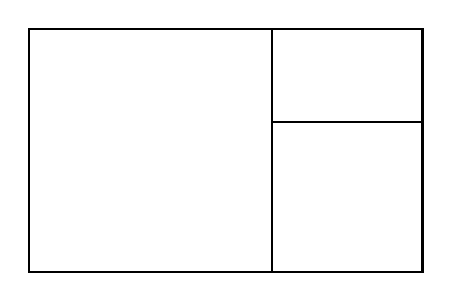
\begin{tikzpicture}
        \draw[thick] (0,0) rectangle (5,3.09); % Golden rectangle
        \draw[thick] (3.09,0) rectangle (5,3.09); % Square
        \draw[thick] (3.09,1.91) rectangle (5,3.09); % Smaller rectangle
    \end{tikzpicture}
    \caption{The 'Golden Rectangle'}
\end{figure}
The Golden Ratio has several interesting properties:
\begin{itemize}
    \item The Golden Ratio can be expressed as a continued fraction:
    \[
        \phi = 1 + \frac{1}{1 + \frac{1}{1 + \frac{1}{1 + \cdots}}}.
    \]
    \item The Golden Ratio satisfies the equation:
    \[
        \phi^2 = \phi + 1.
    \]
    \item The reciprocal of the Golden Ratio is equal to the Golden Ratio minus one:
    \[
        \frac{1}{\phi} = \phi - 1.
    \]
    \item The ratio of consecutive Fibonacci numbers approaches the Golden Ratio as $n$ approaches infinity:
    \[
        \lim_{n \to \infty} \frac{F_{n+1}}{F_n} = \phi.
    \]
\end{itemize}


\chapter{The Connection Between Fibonacci Sequence and Golden Ratio}
\section{Ratio of Consecutive Fibonacci Numbers}
\section{Fibonacci Numbers in Nature}

\chapter{Algebraic Properties of the Fibonacci Sequence}
The Fibonacci sequence shows a range of interesting algebraic properties, which find applications in various fields of mathematics and computer science. In this chapter, we will explore some of these properties.
\section{Conversion from Recurrence to Closed Form}
\subsection{Binet's Formula}
It is often useful to express the Fibonacci sequence in a closed form, rather than as a recurrence relation. Binet's formula provides such a closed form expression for the $n^{th}$ Fibonacci number. To derive such a closed form relation, we must explore a few properties of recurrence relations.  \\
\begin{mydefinition}{Linear Homogeneous Recurrence Relation with Constant Coefficients}
    A recurrence relation of the form:
    \[
        a_n = c_1 a_{n-1} + c_2 a_{n-2} + \cdots + c_k a_{n-k}
    \]
    where $c_1, c_2, \ldots, c_k$ are constants and $c_k \neq 0$, is called a linear homogeneous recurrence relation with constant coefficients.
\end{mydefinition}
\begin{mydefinition}{Order of a Recurrence Relation}
    The order of a recurrence relation is the number of previous terms used to define the current term. In the case of a linear homogeneous recurrence relation with constant coefficients, the order is $k$.
\end{mydefinition}
The Fibonacci sequence is a linear homogeneous recurrence relation with constant coefficients, where $c_1 = 1$ and $c_2 = 1$. \\
Moreover, the Fibonacci sequence is of order $2$, as each term is defined in terms of the two preceding terms. \\
\begin{mydefinition}{Characteristic Equation}
    The characteristic equation of a linear homogeneous recurrence relation with constant coefficients is obtained by replacing $a_n$ with $x^n$, $a_{n-1}$ with $x^{n-1}$, and so on, leading to the polynomial equation:
    \[
        x^k - c_1 x^{k-1} - c_2 x^{k-2} - \cdots - c_k = 0.
    \]
\end{mydefinition}
In the case of the Fibonacci sequence, the characteristic equation is:
\[
    x^2 - x - 1 = 0
\]
\begin{mytheorem}{General Solution of Linear Homogeneous Recurrence Relation}
    The general solution of a linear homogeneous recurrence relation with constant coefficients can be expressed in terms of the roots of its characteristic equation. If the characteristic equation has distinct roots $r_1, r_2, \ldots, r_k$, then the general solution is given by:
    \[
        a_n = A_1 r_1^n + A_2 r_2^n + \cdots + A_k r_k^n
    \]
    where $A_1, A_2, \ldots, A_k$ are constants determined by the initial conditions of the recurrence relation.
\end{mytheorem}
\begin{proof}
    Suppose the characteristic equation has $k$ distinct roots $r_1, r_2, \ldots, r_k$. We will show that the sequence defined by:
    \[
        a_n = A_1 r_1^n + A_2 r_2^n + \cdots + A_k r_k^n
    \]
    satisfies the recurrence relation. To do this, we will substitute this expression into the left-hand side of the recurrence relation and show that it equals the right-hand side. \\
    First, we compute $a_{n-1}$ and $a_{n-2}$:
    \[
        a_{n-1} = A_1 r_1^{n-1} + A_2 r_2^{n-1} + \cdots + A_k r_k^{n-1}
    \]
    \[
        a_{n-2} = A_1 r_1^{n-2} + A_2 r_2^{n-2} + \cdots + A_k r_k^{n-2}
    \]
    Now, we substitute these expressions into the left-hand side of the recurrence relation:
    \[
        a_n = c_1 a_{n-1} + c_2 a_{n-2}
    \]
    This gives us:
    \[
        A_1 r_1^n + A_2 r_2^n + \cdots + A_k r_k^n = c_1 (A_1 r_1^{n-1} + A_2 r_2^{n-1} + \cdots + A_k r_k^{n-1}) + c_2 (A_1 r_1^{n-2} + A_2 r_2^{n-2} + \cdots + A_k r_k^{n-2})
    \]
    Since $r_i$ are roots of the characteristic equation, we have:
    \[
        c_1 r_i + c_2 = r_i^2
    \]
    for each $i$. Substituting this into our equation, we find that the left-hand side equals the right-hand side, thus proving the claim. The same proof can be extended to recurrence relations of higher order whose characteristic equations have distinct roots. \\
    Finally, the constants $A_1, A_2, \ldots, A_k$ can be determined by using the initial conditions of the recurrence relation.
\end{proof}
\noindent
Using the above theorem, we can derive Binet's formula for the Fibonacci sequence. 
\subsubsection{Derivation of Binet's Formula}
We start with the characteristic equation of the Fibonacci recurrence relation:
\[
    x^2 = x + 1
\]
The solutions to this equation are:
\[
    \alpha = \frac{1 + \sqrt{5}}{2} \quad \text{and} \quad \beta = \frac{1 - \sqrt{5}}{2}.
\]
The general solution to the recurrence relation can be expressed as:
\[
    F_n = A \alpha^n + B \beta^n
\]
for some constants $A$ and $B$. To determine these constants, we use the initial conditions of the Fibonacci sequence:
\[    F_0 = 0 \quad \text{and} \quad F_1 = 1
\]
Substituting $n = 0$ into the general solution, we get:
\[    F_0 = A + B = 0 \quad \Rightarrow \quad B = -A
\]
Substituting $n = 1$ into the general solution, we get:
\[    F_1 = A \alpha + B \beta = A \alpha - A \beta = A(\alpha - \beta) = 1
\]
Since $\alpha - \beta = \sqrt{5}$, we have:
\[    A \sqrt{5} = 1 \quad \Rightarrow \quad A = \frac{1}{\sqrt{5}} \quad \text{and} \quad B = -\frac{1}{\sqrt{5}}
\]
Thus, the closed form expression for the $n^{th}$ Fibonacci number, known as Binet's formula, is given by:
\[
    F_n = \frac{1}{\sqrt{5}} \left( \left( \frac{1 + \sqrt{5}}{2} \right)^n - \left( \frac{1 - \sqrt{5}}{2} \right)^n \right)
\]
This can be represented more compactly as:
\[
    F_n = \frac{\phi^n - (1 - \phi)^n}{\sqrt{5}}
\]
where $\phi = \frac{1 + \sqrt{5}}{2}$ is the Golden Ratio.
\section{Matrix Representation of the Fibonacci Sequence}
The Fibonacci sequence can also be represented using matrix exponentiation. This provides an efficient way to compute Fibonacci numbers, especially for large $n$, and has applications in computer science and algorithm design.
\subsection{Matrix Formulation}
Suppose we have a linear operator $T : \R^2 \to \R^2$ such that: 
$$T(\begin{bmatrix}F_n \\ F_{n-1} \end{bmatrix}) = \begin{bmatrix}F_{n+1} \\ F_n \end{bmatrix}$$
Let us determine the matrix representation of $T$. Let us use the standard basis vectors of $\R^2$, $e_1 = \begin{bmatrix}1 \\ 0 \end{bmatrix}$ and $e_2 = \begin{bmatrix}0 \\ 1 \end{bmatrix}$. We have:
\begin{align*}
    T(e_1) &= T(\begin{bmatrix}1 \\ 0 \end{bmatrix}) = \begin{bmatrix}F_1 \\ F_0 \end{bmatrix} = \begin{bmatrix}1 \\ 0 \end{bmatrix} = 1e_1 + 0e_2, \\
    T(e_2) &= T(\begin{bmatrix}0 \\ 1 \end{bmatrix}) = \begin{bmatrix}F_2 \\ F_1 \end{bmatrix} = \begin{bmatrix}1 \\ 1 \end{bmatrix} = 1e_1 + 1e_2.
\end{align*}
Thus, the matrix representation of $T$ is given by:
\[
    [T] = \begin{bmatrix}1 & 1 \\ 1 & 0 \end{bmatrix}
\]
\subsection{Computing Fibonacci Numbers using Matrix Exponentiation}
Using the matrix representation of the linear operator $T$, we can express the Fibonacci numbers in terms of matrix exponentiation. Specifically, we have:
\[
    \begin{bmatrix}F_n \\ F_{n-1} \end{bmatrix} = T^{n-1} \begin{bmatrix}F_1 \\ F_0 \end{bmatrix} = T^{n-1} \begin{bmatrix}1 \\ 0 \end{bmatrix}
\]
Thus, to compute the $n^{th}$ Fibonacci number, we can compute the $(1,1)$ entry of the matrix $T^{n-1}$. \\
Matrix exponentiation can be performed efficiently using the method of exponentiation by squaring, which allows us to compute $T^{n-1}$ in $O(\log n)$ time. This is significantly faster than the naive recursive or iterative methods, especially for large values of $n$. \\
\subsection{Interesting Group Theoretic Properties}
\begin{mydefinition}{Group}
    A group is a set $G$ equipped with a binary operation $\cdot : G \times G \to G$ that satisfies the following properties:
    \begin{itemize}
        \item \textbf{Closure:} For all $a, b \in G$, the result of the operation $a \cdot b$ is also in $G$.
        \item \textbf{Associativity:} For all $a, b, c \in G$, we have $(a \cdot b) \cdot c = a \cdot (b \cdot c)$.
        \item \textbf{Identity Element:} There exists an element $e \in G$ such that for all $a \in G$, we have $e \cdot a = a \cdot e = a$.
        \item \textbf{Inverse Element:} For each element $a \in G$, there exists an element $b \in G$ such that $a \cdot b = b \cdot a = e$, where $e$ is the identity element.
    \end{itemize}
\end{mydefinition}
\begin{mydefinition}{Isomorphism of Groups}
    An isomorphism between two groups $(G, \cdot)$ and $(H, *)$ is a bijective function $\phi : G \to H$ such that for all $a, b \in G$, we have:
    \[
        \phi(a \cdot b) = \phi(a) * \phi(b).
    \]
\end{mydefinition}
The matrix representation of the Fibonacci sequence also reveals interesting group theoretic properties. The set of matrices of the form:
\[
    \begin{bmatrix}F_{n+1} & F_n \\ F_n & F_{n-1} \end{bmatrix}
\]
for $n \geq 0$ forms a group under matrix multiplication. This group is isomorphic to the group of integers under addition, with the isomorphism given by the mapping:
\[
    n \mapsto \begin{bmatrix}F_{n+1} & F_n \\ F_n & F_{n-1} \end{bmatrix}
\]
This group structure provides a deeper understanding of the algebraic properties of the Fibonacci sequence and its connections to other areas of mathematics, such as number theory and combinatorics.
\begin{mytheorem}{The Fibonacci Matrix Group}
    The set of matrices of the form:
    \[
        \begin{bmatrix}F_{n+1} & F_n \\ F_n & F_{n-1} \end{bmatrix}
    \]
    for $n \geq 0$ forms a group under matrix multiplication, which is isomorphic to the group of integers under addition.
\end{mytheorem}
\begin{proof}
    To show that the set of matrices of the form:
    \[
        M_n = \begin{bmatrix}F_{n+1} & F_n \\ F_n & F_{n-1} \end{bmatrix}
    \]
    for $n \geq 0$ forms a group under matrix multiplication, we need to verify the group properties: closure, associativity, identity element, and inverse element. \\
    \textbf{Closure:} Let $M_m$ and $M_n$ be two matrices in the set. We need to show that their product $M_m M_n$ is also in the set. We have:
    \[
        M_m M_n = \begin{bmatrix}F_{m+1} & F_m \\ F_m & F_{m-1} \end{bmatrix} \begin{bmatrix}F_{n+1} & F_n \\ F_n & F_{n-1} \end{bmatrix}
    \]
    Performing the matrix multiplication, we get:
    \[
        = \begin{bmatrix}F_{m+1}F_{n+1} + F_m F_n & F_{m+1}F_n + F_m F_{n-1} \\ F_m F_{n+1} + F_{m-1}F_n & F_m F_n + F_{m-1}F_{n-1} \end{bmatrix}
    \]
    Using the Fibonacci recurrence relation, we can simplify this to:
    \[
        = \begin{bmatrix}F_{m+n+1} & F_{m+n} \\ F_{m+n} & F_{m+n-1} \end{bmatrix}
    \]
    Thus, $M_m M_n = M_{m+n}$, which is in the set. Therefore, closure holds. \\
    \textbf{Associativity:} Matrix multiplication is associative, so for any matrices $M_a$, $M_b$, and $M_c$ in the set, we have:
    \[
        (M_a M_b) M_c = M_a (M_b M_c).
    \]
    Thus, associativity holds. \\
    \textbf{Identity Element:} The identity matrix in this set is:
    \[
        M_0 = \begin{bmatrix}F_1 & F_0 \\ F_0 & F_{-1} \end{bmatrix} = \begin{bmatrix}1 & 0 \\ 0 & 1 \end{bmatrix}
    \]
    since $F_1 = 1$, $F_0 = 0$, and $F_{-1} = 1$. For any matrix $M_n$ in the set, we have:
    \[
        M_n M_0 = M_0 M_n = M_n.
    \]
    Thus, the identity element exists. \\
    \textbf{Inverse Element:} For each matrix $M_n$, we need to find a matrix $M_{-n}$ such that:
    \[        M_n M_{-n} = M_{-n} M_n = M_0.
    \]
\end{proof}
\section{Generating Functions}
\chapter{Topological Properties of the Fibonacci Sequence}
\section{Periodic and Quasi-Periodic Properties}
\subsection{The Quasi-Periodic Nature of the Fibonacci Sequence}
The significance of the quasi-periodic nature of the Fibonacci sequence lies in its ability to exhibit patterns and structures that are not strictly periodic but still possess a form of regularity. This property has implications in various fields, including number theory, combinatorics, and even physics, where quasi-periodic structures can arise in the study of quasicrystals and other complex systems.
\begin{mydefinition}{Quasi-Periodicity}
    A sequence $(a_n)$ is said to be quasi-periodic if there exists a positive integer $p$ such that for all integers $n$, the difference $a_{n+p} - a_n$ is bounded. 
\end{mydefinition}
\begin{mytheorem}[Quasi-Periodicity of the Fibonacci Sequence]
    The Fibonacci sequence $(F_n)$ is quasi-periodic. 
\end{mytheorem}
\begin{proof}
    To show that the Fibonacci sequence is quasi-periodic, we need to find a positive integer $p$ such that for all integers $n$, the difference $F_{n+p} - F_n$ is bounded. Let us choose $p = 5$. We will show that the difference $F_{n+5} - F_n$ is bounded for all integers $n$. \\
    Using the Fibonacci recurrence relation, we can express $F_{n+5}$ in terms of $F_n$ and the next four Fibonacci numbers:
    \[    F_{n+5} = F_{n+4} + F_{n+3} = (F_{n+3} + F_{n+2}) + F_{n+3} = 2F_{n+3} + F_{n+2}
\] 
    Continuing this process, we can express $F_{n+5}$ as a linear combination of $F_n$ and $F_{n+1}$:
    \[    F_{n+5} = 5F_n + 3F_{n+1}
\]
    Since the Fibonacci numbers grow exponentially, we can see that the difference $F_{n+5} - F_n$ is bounded by a constant multiple of $F_n$. Specifically, we have:
    \[
        |F_{n+5} - F_n| \leq C \cdot F_n
    \]
    for some constant $C$. Thus, the difference $F_{n+5} - F_n$ is bounded for all integers $n$. Therefore, the Fibonacci sequence is quasi-periodic with period $p = 5$.
\end{proof}
\begin{mynote}
    The choice of $p = 5$ is not unique; other values of $p$ can also be used to demonstrate the quasi-periodicity of the Fibonacci sequence. The key idea is that the differences between terms in the sequence can be expressed in terms of a finite number of preceding terms, leading to bounded differences over fixed intervals.
\end{mynote}
\begin{example}
    The Fibonacci sequence $(F_n)$ is quasi-periodic with period $p = 5$. For example, consider the first few terms of the Fibonacci sequence:
    \[
        F_0 = 0, \quad F_1 = 1, \quad F_2 = 1, \quad F_3 = 2, \quad F_4 = 3, \quad F_5 = 5, \quad F_6 = 8, \quad F_7 = 13, \quad F_8 = 21, \quad F_9 = 34.
    \]
    We can compute the differences $F_{n+5} - F_n$ for $n = 0, 1, 2, 3, 4$:
    \[        F_5 - F_0 = 5 - 0 = 5, \]
    \[        F_6 - F_1 = 8 - 1 =  7, \]
    \[        F_7 - F_2 = 13 - 1 = 12, \]
    \[        F_8 - F_3 = 21 - 2 = 19, \]
    \[        F_9 - F_4 = 34 - 3 = 31. \]
    We can see that the differences $F_{n+5} - F_n$ are bounded by a constant multiple of $F_n$. Thus, the Fibonacci sequence is quasi-periodic with period $p = 5$.
\end{example}
\subsection{Pisano Periods}
The Fibonacci sequence modulo $m$ exhibits periodic behavior. This periodicity is characterized by the Pisano period, which is the length of the cycle of Fibonacci numbers modulo $m$. The Pisano period has been studied extensively and has applications in number theory and cryptography.
\begin{mytheorem}
    The sequence of Fibonacci numbers modulo $m$ is periodic for any positive integer $m$, i.e. $\{F_n \mod m\}_{n\geq 0}$ is a periodic sequence.
\end{mytheorem}
\begin{proof}
    We know that the Fibonacci Sequnce is generated by the matrix: 
    \[
    \begin{bmatrix}
    F_{n+1} & F_n \\
    F_n & F_{n-1}
    \end{bmatrix} = \begin{bmatrix}1 & 1 \\
    1 & 0
    \end{bmatrix}^n \begin{bmatrix}F_1 \\ F_0 \end{bmatrix}
    \]
    We know that the matrix is an element of $GL_2(\mathbb{Z}/m\mathbb{Z})$, the group of invertible $2\times 2$ matrices with entries in $\mathbb{Z}/m\mathbb{Z}$. Since $GL_2(\mathbb{Z}/m\mathbb{Z})$ is a finite group, the powers of the matrix must eventually repeat. Thus, there exist integers $k$ and $l$ such that:
    \[
        \begin{bmatrix}1 & 1 \\ 1 & 0 \end{bmatrix}^k \equiv \begin{bmatrix}1 & 1 \\ 1 & 0 \end{bmatrix}^l \mod m
    \]
    This implies that:
    \[
        F_{n+k} \equiv F_{n+l} \mod m
    \]
    for all integers $n$. Therefore, the sequence of Fibonacci numbers modulo $m$ is periodic.
\end{proof}
\begin{mynote}
    The Pisano period $\pi(m)$ is the length of the cycle of Fibonacci numbers modulo $m$. For example, the Pisano period for $m = 2$ is $3$, as the sequence of Fibonacci numbers modulo $2$ is:
    \[
        0, 1, 1, 0, 1, 1, 0, \ldots
    \]
    which repeats every $3$ terms. Similarly, the Pisano period for $m = 3$ is $8$, as the sequence of Fibonacci numbers modulo $3$ is:
    \[
        0, 1, 1, 2, 0, 2, 2, 1, 0, \ldots
    \]
    which repeats every $8$ terms.
\end{mynote}

\begin{mytheorem}[Quasi-Periodicity of Fibonacci Sequence Modulo m]
    The Fibonacci sequence $(F_n)$ is quasi-periodic modulo $m$ for any positive integer $m$.
\end{mytheorem}
\begin{proof}
    To show that the Fibonacci sequence is quasi-periodic modulo $m$, we need to find a positive integer $p$ such that for all integers $n$, the difference $F_{n+p} \mod m - F_n \mod m$ is bounded. \\
    The Fibonacci sequence modulo $m$ is periodic, with a period known as the Pisano period, denoted by $\pi(m)$. This means that:
    \[
        F_{n+\pi(m)} \mod m = F_n \mod m
    \]
    for all integers $n$. Therefore, we can choose $p = \pi(m)$. Then, for all integers $n$, we have:
    \[
        F_{n+p} \mod m - F_n \mod m = F_{n+\pi(m)} \mod m - F_n \mod m = 0.
    \]
    Thus, the difference $F_{n+p} \mod m - F_n \mod m$ is bounded (in fact, it is zero) for all integers $n$. Therefore, the Fibonacci sequence is quasi-periodic modulo $m$ with period $p = \pi(m)$.
\end{proof}

\section{Fibonacci Sequence as a Topological Space}
\begin{mydefinition}{Topological Space}
    A topological space is a set $X$ equipped with a collection $\tau$ of subsets of $X$ satisfying the following properties:
    \begin{itemize}
        \item The empty set and the entire set $X$ are in $\tau$.
        \item The union of any collection of sets in $\tau$ is also in $\tau$.
        \item The intersection of any finite collection of sets in $\tau$ is also in $\tau$.
    \end{itemize}
    The collection $\tau$ is called a topology on $X$, and the sets in $\tau$ are called open sets.
\end{mydefinition}
\begin{example}
    The set of real numbers $\R$ with the standard topology, where the open sets are defined as open intervals $(a, b)$ for $a, b \in \R$, is a topological space.
\end{example}
\begin{mydefinition}{Fibonacci Topological Space}
    The Fibonacci topological space is defined as the set of Fibonacci numbers $\{F_n : n \geq 0\}$ equipped with the topology generated by the basis consisting of all open intervals $(F_n - \epsilon, F_n + \epsilon)$ for each Fibonacci number $F_n$ and for all $\epsilon > 0$.
\end{mydefinition}
\begin{mytheorem}[The Fibonacci Numbers with the Fibonacci Topology Form a Topological Space]
    The set of Fibonacci numbers $\{F_n : n \geq 0\}$ with the Fibonacci topology is a topological space.
\end{mytheorem}
\begin{proof}
    To show that the set of Fibonacci numbers $\{F_n : n \geq 0\}$ with the Fibonacci topology is a topological space, we need to verify the three properties of a topology. \\
    \textbf{Property 1:} The empty set and the entire set $\{F_n : n \geq 0\}$ are in the topology. \\
    The empty set is trivially in the topology. The entire set $\{F_n : n \geq 0\}$ can be expressed as the union of all open intervals $(F_n - \epsilon, F_n + \epsilon)$ for each Fibonacci number $F_n$ and for all $\epsilon > 0$. Thus, the entire set is also in the topology. \\
    \textbf{Property 2:} The union of any collection of sets in the topology is also in the topology. \\
    Let $\{U_i\}_{i \in I}$ be a collection of open sets in the Fibonacci topology. Each $U_i$ can be expressed as a union of open intervals $(F_n - \epsilon, F_n + \epsilon)$. The union $\bigcup_{i \in I} U_i$ can then be expressed as a union of these open intervals, which is also an open set in the Fibonacci topology. Thus, the union of any collection of sets in the topology is also in the topology. \\
    \textbf{Property 3:} The intersection of any finite collection of sets in the topology is also in the topology. \\
    Let $U_1, U_2, \ldots, U_k$ be a finite collection of open sets in the Fibonacci topology. Each $U_j$ can be expressed as a union of open intervals $(F_n - \epsilon, F_n + \epsilon)$. The intersection $\bigcap_{j=1}^{k} U_j$ can then be expressed as a finite intersection of these open intervals. Since the intersection of a finite number of open intervals is also an open interval (or empty), it follows that the intersection $\bigcap_{j=1}^{k} U_j$ is also an open set in the Fibonacci topology. Thus, the intersection of any finite collection of sets in the topology is also in the topology. \\
    Since all three properties of a topology are satisfied, we conclude that the set of Fibonacci
\end{proof}



\section{Convergence of Ratios of Consecutive Fibonacci Numbers}
\section{Fibonacci Sequence and the Golden Spiral}

\chapter{Combinatoric and Computer Science Applications of the Fibonacci Sequence}
\section{Combinatoric Properties}
\subsection{Counting Problems Involving Fibonacci Numbers}
\subsubsection{Tiling Problems}
The Fibonacci sequence appears in various counting problems in combinatorics. One classic example is counting the number of ways to tile a $2 \times n$ board using $1 \times 2$ dominoes and $2 \times 1$ dominoes. The number of ways to tile such a board is given by the $n^{th}$ Fibonacci number. \\
To see why this is the case, consider the following reasoning:
\begin{itemize}
    \item If we place a vertical domino in the first column, we are left with a $2 \times (n-1)$ board to tile. The number of ways to tile this smaller board is $F_{n-1}$.
    \item If we place two horizontal dominoes in the first two rows of the first two columns, we are left with a $2 \times (n-2)$ board to tile. The number of ways to tile this smaller board is $F_{n-2}$.
\end{itemize}
Thus, the total number of ways to tile a $2 \times n$ board is given by the recurrence relation:
\[    T(n) = T(n-1) + T(n-2)
\]
with initial conditions $T(1) = 1$ and $T(2) = 2$. This is precisely the Fibonacci recurrence relation, and hence we have:
\[    T(n) = F_n
\]
Lets consider the figure below which illustrates the tiling of a $2 \times 5$ board:
\begin{figure}[H]
    \centering
    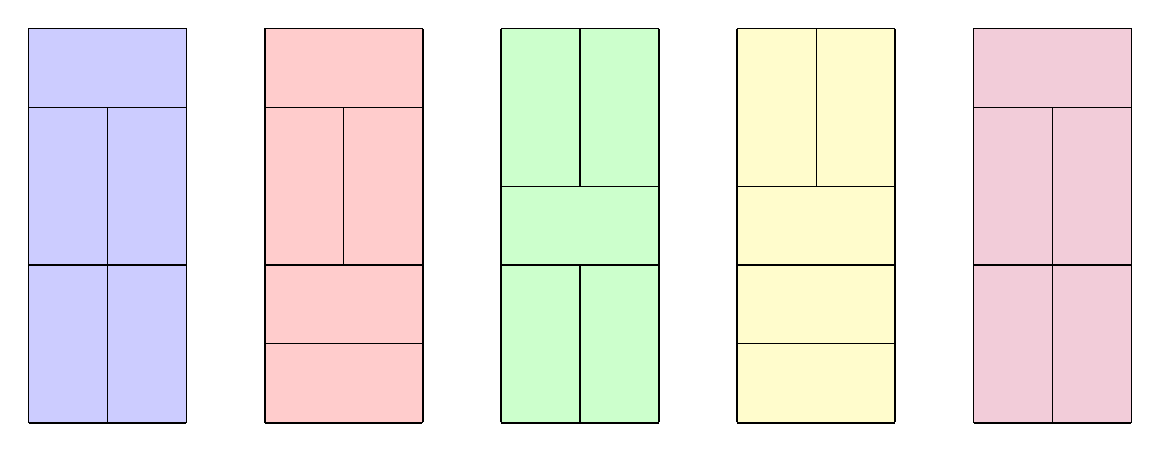
\begin{tikzpicture}
        \draw[thick] (0,0) grid (2,5);
        \draw[thick] (3,0) grid (5,5);
        \draw[thick] (6,0) grid (8,5);
        \draw[thick] (9,0) grid (11,5);
        \draw[thick] (12,0) grid (14,5);
        % First Tiling
        \draw[fill=blue!20] (0,0) rectangle (1,2);
        \draw[fill=blue!20] (1,0) rectangle (2,2);
        \draw[fill=blue!20] (0,2) rectangle (1,4);
        \draw[fill=blue!20] (1,2) rectangle (2,4);
        \draw[fill=blue!20] (0,4) rectangle (2,5);
        % Second Tiling
        \draw[fill=red!20] (3,0) rectangle (5,1);
        \draw[fill=red!20] (3,1) rectangle (5,2);
        \draw[fill=red!20] (3,2) rectangle (4,4);
        \draw[fill=red!20] (4,2) rectangle (5,4);
        \draw[fill=red!20] (3,4) rectangle (5,5);
        % Third Tiling
        \draw[fill=green!20] (6,0) rectangle (7,2);
        \draw[fill=green!20] (7,0) rectangle (8,2);
        \draw[fill=green!20] (6,2) rectangle (8,3);
        \draw[fill=green!20] (6,3) rectangle (8,5);
        \draw[fill=green!20] (7,3) rectangle (8,5);
        % Fourth Tiling
        \draw[fill=yellow!20] (9,0) rectangle (11,1);
        \draw[fill=yellow!20] (9,1) rectangle (11,3);
        \draw[fill=yellow!20] (9,3) rectangle (10,5);
        \draw[fill=yellow!20] (10,3) rectangle (11,5);
        \draw[fill=yellow!20] (9,2) rectangle (11,3);
        % Fifth Tiling
        \draw[fill=purple!20] (12,0) rectangle (14,2);
        \draw[fill=purple!20] (12,2) rectangle (13,5);
        \draw[fill=purple!20] (13,0) rectangle (14,2);
        \draw[fill=purple!20] (13,2) rectangle (14,4);
        \draw[fill=purple!20] (12,4) rectangle (14,5);  
    \end{tikzpicture}
    \caption{Tiling of a $2 \times 5$ Board}
    \label{fig:tiling}
\end{figure}
\subsubsection{Binary Strings without Consecutive 1s}
Another combinatorial problem that involves Fibonacci numbers is counting the number of binary strings of length $n$ that do not contain consecutive 1s. The number of such binary strings is given by the $(n+2)^{th}$ Fibonacci number. \\
To see why this is the case, consider the following reasoning:
\begin{itemize}
    \item If the first digit of the binary string is 0, the remaining $n-1$ digits can be any valid binary string of length $n-1$. The number of such strings is $F_{n+1}$.
    \item If the first digit of the binary string is 1, the second digit must be 0 (to avoid consecutive 1s), and the remaining $n-2$ digits can be any valid binary string of length $n-2$. The number of such strings is $F_n$.
\end{itemize}
Thus, the total number of binary strings of length $n$ without consecutive 1s is given by the recurrence relation:
\[    B(n) = B(n-1) + B(n-2)
\]
with initial conditions $B(1) = 2$ and $B(2) = 3$. This is also a Fibonacci-like sequence, and we have:
\[    B(n) = F_{n+2}
\]

\section{Applications in Computer Science}
\subsection{Fibonacci Heap Data Structure}
Fibonacci heaps are a type of priority queue data structure that take advantage of the Fibonacci sequence to achieve better amortized time complexities for certain operations. They are particularly useful in network optimization algorithms, such as Dijkstra's shortest path algorithm.
\section{Simulations and Modeling}
\subsection{Fractal Generation}
The Fibonacci sequence can be used to generate fractal patterns, such as the Fibonacci spiral. This spiral is created by drawing quarter-circle arcs connecting the opposite corners of squares with side lengths equal to Fibonacci numbers. The resulting pattern exhibits self-similarity and is often found in nature, such as in the arrangement of leaves and the structure of shells.
The python code below generates a Fibonacci spiral using the turtle graphics library:


\end{document}
